\setchapterpreamble[ur][.6\textwidth]{%
\dictum[Fyodor Dostoyevsky, \textit{The Idiot} (1868--9)]{%
One can't understand everything at once, we can't begin with perfection all at once! In order to reach perfection one must begin by being ignorant of a great deal. And if we understand things too quickly, perhaps we shan't understand them thoroughly.}\vskip1em

\dictum[Voltaire a.k.a. Fran\c{c}ois-Marie Arouet, \textit{Candide} (1759)]{%
Si nous ne trouvons pas des choses agr\'eables, nous trouverons du moins des choses nouvelles.}\vskip1em}

\chapter[Chapter 1: General introduction]{General introduction}
\chaptermark{General introduction}
%%%%%%%%%%%%%%%%%%%%%%%%%%%%%%%%%%%%%%%%%%%%%%%%%%%%%%%%%%%%%%%%%%%%%%%%%%%%%%%%%%%%%%

%%%%%%%%%%%%%%%%%%%%%%%%%%%%%%%%%%%%%%%%%%%
\section{Variation in fitness}
\subsection{The idea of variation in evolutionary biology}
Understanding variation among living beings is at the heart of evolutionary questioning. It is in fact its very starting point. Darwin opens his book \emph{the Origin of Species} with two chapters describing variability in domestic and wild organisms \parencite{Darwin1859}.
Building on these observations, Darwin then summarizes the evidence showing that variation within species is the fuel generating the astonishing diversity among species\textemdash thus clarifying what species are and are not \parencite[][pp. 129-163]{Wilkins2009}\textemdash but also the striking fit between most organisms and their environment.

These great answers immediately opened many more questions, some of which still keep scientists busy more than 150 years later. In particular, nineteenth century biologists struggled with the sources of variation within species. Of course, the effect of ageing was acknowledged and a great deal of attention was paid to the effect of the environment, although the mechanisms of both remained obscure. 
But Darwinian arguments build on the observation of this special kind of inherited variation that can appear among siblings of a same litter, clutch or pod, and that is subsequently transmitted from parent to offspring \parencite[][Chapter 1]{Darwin1859}. The late nineteenth century was utterly ignorant of the sources of inherited variation within species. Only at the beginning of the twentieth century were the laws of inheritance progressively discovered and spread to the scientific community (e.g. by Mendel, de Vries, Correns and Bateson, none of whom I have read). Four more decades saw these laws formalized into a unified scientific theory \parencite{Fisher1930}, and explained at the molecular level \parencite{Oswald1943, Watson1953}, thus closing the logical gap in Darwin's argument: Relatives resemble each other because they share similar gene versions on long strands of DNA, a molecule that is copied with a very high fidelity and transmitted from parent to offspring; There is variation among siblings because of the reshuffling and segregation of parental genes and  on occasions because DNA mutates. 
Our understanding of within species variation has made terrific progresses and now fits elegantly in the broader evolutionary theory. Still, answers rarely fail to bring new problems and there are still many questions to be refined or newly explored; for instance:
\begin{itemize}
\item How does genetic variation translate into phenotypic variation at the molecular, physiological and behavioural levels? \parencite{Kirschner2010}
\item How do mutations generate innovations without preventing the organism from working? \parencite{Wagner2014} 
\item How often and how strongly is inheritance not mediated by DNA? \parencite{Bonduriansky2012}
\item What are the relative roles of stochastic processes, genes and the environment in generating variation in wild populations? \parencite{Raj2008, Postma2014}
\end{itemize}
These questions, and others, are especially difficult and far-reaching when applied to variation in fitness, a concept that we shall now introduce. 

%fitness
\subsection{Fitness and the special problem of variation in fitness}
There has been a great deal written about the concept of fitness, and as is common for central scientific concepts REF?, its definition is problematic. Actually, there are many definitions, and sub-definitions. 
In this thesis, what we mean by \emph{fitness} is ...
most adapted to the study framework.
with the difficulty that... 

In this thesis, we will not really deal with the fundamental question of appearance and maintenance of variation in fitness (e.g. lek paradox, see XX), but rather with its proximal sources.

Fitness proxy because we cannot directly observe fitness. First must isolate what is fitness in these measures. 



 
%%%%%%%%%%%%%%%%%%%%%%%%%%%%%%%%%%%%%%%%%%%
\section{Quantitative genetics}

How to measure and make sense of genetic variation?
For over a century, there have been two main approaches. 
These can be summarized as ``bottom-up'' and ``top-down''.
The Mendelians and the biometricians

Some pros and cons of both approaches are nicely illustrated by the confrontation of the quantitative genetics of mass with the genotyping of a candidate gene for mass. The latter is a side project of this Ph.D. that does not appear in the other chapters, and we take the opportunity to present it below.

\subsection{A candidate gene for body mass: insights and limits}

We used a candidate gene approach to uncover the molecular mechanisms 
To date, only the candidate gene fully analysed is an intronic region of the gene \emph{lepr}, which codes for the leptin receptor. This hormone is known to regulate fat metabolism, energy expenditure and food intake, including in rodents \parencite{Houseknecht1998}.

We found a recessive allele (let call the recessive allele \emph{a}, and the dominant allele \emph{A}) associated with lighter individuals (Fig. \ref{fig:leprpheno}\textbf{A}). Homozygotes \emph{aa} were -2.9 g lighter (95\% credibility interval $[0.6;5.1]$), that is, 8\% lighter than the mean. On average, during their lifetime, these \emph{aa} individuals produced one third less offspring than the \emph{AA} individuals (Fig. \ref{fig:leprpheno}\textbf{B}). This strong difference in fitness is however not statistically significant, meaning that it could very well be the result of chance alone. These results suggests links between the physiology of the organism, its environment and the causes of natural selection that could not be sensed from the estimation of genetic variances and covariances. 
Genetic variances and covariances are however necessary to 
Based such a strong phenotypic effect, \emph{lepr} could be called a major locus, but how much of the genetic variation does it explain?

\begin{figure}[ht]
	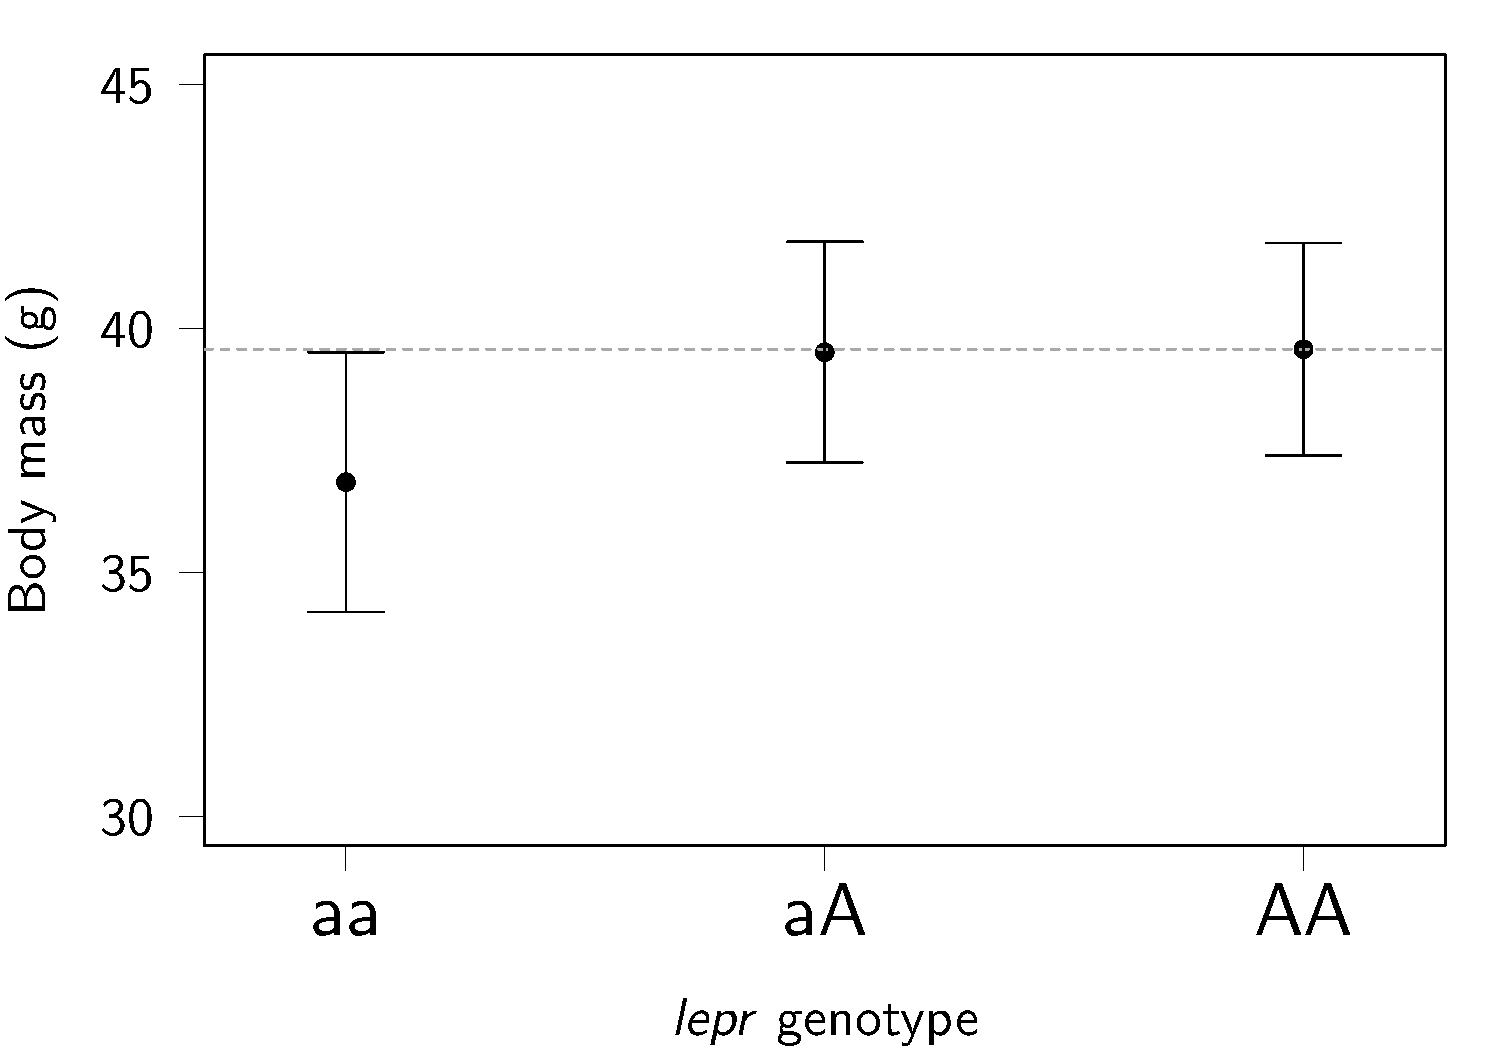
\includegraphics[width=0.5\textwidth]{FiguresGeneral/PhenoEffect-1}
	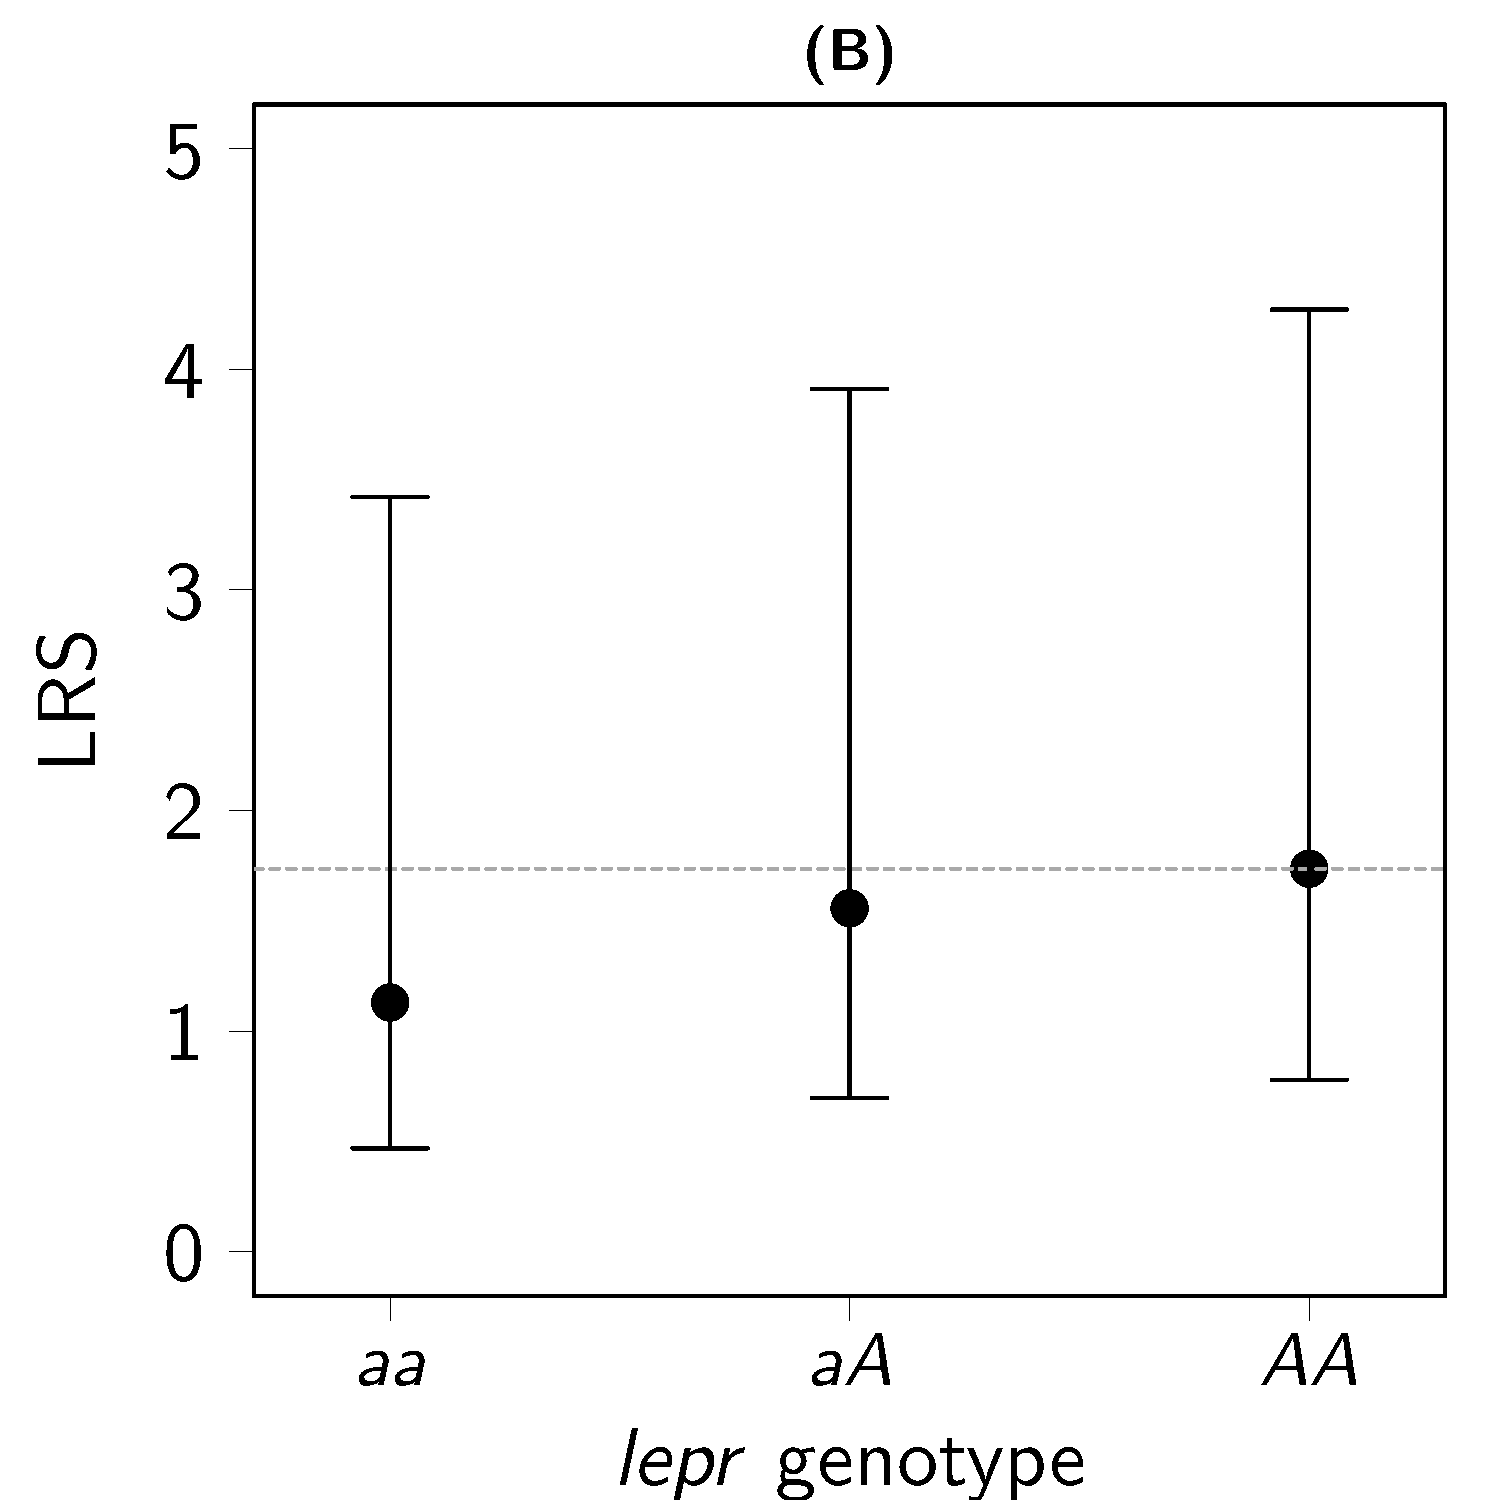
\includegraphics[width=0.5\textwidth]{FiguresGeneral/FitnessEffect-1}
	\caption{Body mass and lifetime reproductive success (LRS) as a function of \emph{lepr} genotypes. 
	(\textbf{A}) Expected body mass of snow voles bearing the three \emph{lepr} genotypes. The expectations and 95\% confidence intervals were predicted from a linear mixed model fitted to the 2311 mass measurement of 532 snow voles. The model accounted for sex, age, date of capture and their two-ways interactions, as well as year of capture and multiple measurements of the same individual.
	(\textbf{B}) Expected LRS of snow voles bearing the three \emph{lepr} genotypes. The expectations and 95\% confidence intervals were predicted from a Poisson generalized linear mixed model fitted to the LRS of 611 snow voles. The model accounted for inbreeding coefficient, year of birth and over-dispersion (using an observation-level random effect). For both panels, the dashed horizontal line projects the expected value of genotype \emph{AA} to ease comparison with \emph{Aa} and \emph{aa}.}
	\label{fig:leprpheno}
\end{figure}

Knowing the effect of the three genotypes and the allele frequencies one can compute analytically the additive genetic variances associated with a bi-allelic locus \parencite[][p77]{Fisher1941average,Lynch1998}. Thus, the additive genetic variances associated with \emph{lepr} are $0.052$  for body mass and $0.006$ for LRS. For both traits, \emph{lepr} explains about 1\% of the additive genetic variation as estimated from an animal model. This is a relatively large proportion for a single locus given that quantitative traits loci typically explain a fraction of a percent to a few percents of V$_\text{A}$, when they have a large enough sample size to mitigate Beavis effect \parencite{Flint2009,Jensen2014}.  Still, 1\% of V$_\text{A}$ is not sufficient to infer the evolutionary potential of the trait.

Could we not use high-throughput sequencing techniques to explain a larger proportion of genetic variation, and at the same time identify the genes associated with phenoytpic variation and selection? 
In theory we could, but in practice this avenue is a laborious and expensive one. The outcome is also uncertain: 
The first objective, estimating genetic variances often requires huge sample sizes and number of markers and in general only a small fraction of V$_\text{A}$ is recovered \parencite{Bloom2013}. For instance, even in the most abundant and best known model organism, humans (\textit{Homo sapiens} Linnaeus, 1758), 
sample sizes of over XXX were necessary to explain 
XX\% of variation in body mass. 
Such progresses were accomplished by increasing sample sizes by several order of magnitude and developing 
Neither can be achieved in small populations of non-model organisms.

The second objective, identifying the genetic mechanisms of variation and selection , in small populations the number of genetic loci that can be identified with statistical significance can be limited by the problem of multiple comparisons, although solutions are emerging . 

%The uncertainty in the estimation of the effect of \emph{lepr} on mass translates into a p-value of $0.01$. Using the widespread arbitrary threshold of $0.05$, If other genetic loci were analysed, using quantitative trait loci mapping or genome wide association


%%%%%%%%%%%%%%%%%%%%%%%%%%%%%%%%%%%%%%%%%%%
\section{This thesis}

\subsection{Objectives}

\subsection{Churwalden snow voles}

\subsection{Thesis outline}

\printbibliography[heading=subbibliography]

